% !TeX root = ./thesis.tex
% !TeX spellcheck = hu_HU
% !TeX encoding = UTF-8
% !TeX program = pdflatex
% !BIB program = bibtex
%TODO Change language to en_GB (recommended) or en_US for English documents
\documentclass[11pt,a4paper,oneside]{report}             % Egyoldalas (javasolt)
%\documentclass[11pt,a4paper,twoside,openright]{report}  % Duplex

% thanks to http://tex.stackexchange.com/a/47579/71109
\usepackage{ifxetex}
\usepackage{ifluatex}
\newif\ifxetexorluatex % a new conditional starts as false
\ifnum 0\ifxetex 1\fi\ifluatex 1\fi>0
   \xetexorluatextrue
\fi

\ifxetexorluatex
  \usepackage{fontspec}
\else
  \usepackage[T1]{fontenc}
  \usepackage[utf8]{inputenc}
  \usepackage[lighttt]{lmodern}
\fi

\usepackage[english,magyar]{babel} % Alapértelmezés szerint utoljára definiált nyelv lesz aktív, de később külön beállítjuk az aktív nyelvet.

%\usepackage{cmap}
\usepackage{amsfonts,amsmath,amssymb} % Mathematical symbols.
%\usepackage[ruled,boxed,resetcount,linesnumbered]{algorithm2e} % For pseudocodes. % beware: this is not compatible with LuaLaTeX, see http://tex.stackexchange.com/questions/34814/lualatex-and-algorithm2e
\usepackage{booktabs} % For publication quality tables for LaTeX
\usepackage{graphicx}

%\usepackage{fancyhdr}
%\usepackage{lastpage}

\usepackage{anysize}
%\usepackage{sectsty}
\usepackage{setspace} % For setting line spacing

\usepackage[unicode]{hyperref} % For hyperlinks in the generated document.
\usepackage{xcolor}
\usepackage{listings} % For source code snippets.

\usepackage[amsmath,thmmarks]{ntheorem} % Theorem-like environments.

\usepackage[hang]{caption}

\usepackage[list=true]{subcaption}	%tof url
\usepackage{tocloft}

\usepackage{datetime2}

\singlespacing

\newcommand{\selecthungarian}{
	\selectlanguage{magyar}
	\setlength{\parindent}{2em}
	\setlength{\parskip}{0em}
	\frenchspacing
}

\newcommand{\selectenglish}{
	\selectlanguage{english}
	\setlength{\parindent}{0em}
	\setlength{\parskip}{0.5em}
	\nonfrenchspacing
	\renewcommand{\figureautorefname}{Figure}
	\renewcommand{\tableautorefname}{Table}
	\renewcommand{\partautorefname}{Part}
	\renewcommand{\chapterautorefname}{Chapter}
	\renewcommand{\sectionautorefname}{Section}
	\renewcommand{\subsectionautorefname}{Section}
	\renewcommand{\subsubsectionautorefname}{Section}
}

\usepackage[numbers]{natbib}
\usepackage{xspace}

\usepackage{url}
\usepackage{multicol} %stuff side by side
\usepackage[export]{adjustbox} %for alignment
\usepackage{setspace} %for line spacing
\usepackage[section]{placeins} %for placing float inside their section

% Ide teheted a packageket amiket használni szeretnél



%TODO Saját adataiddal töltsd ki a kommentek szerint
%--------------------------------------------------------------------------------------
\newcommand{\szerzoVezeteknev}{Lengyel}
\newcommand{\szerzoKeresztnev}{Márk}
\newcommand{\szerzoNeptun}{LNXQYO}

\newcommand{\szakirany}{\merninf{}} % automat vagy infokom

\newcommand{\konzulensAMegszolitas}{}
\newcommand{\konzulensAVezeteknev}{Hollósi}
\newcommand{\konzulensAKeresztnev}{János}
\newcommand{\konzulensBMegszolitas}{}
\newcommand{\konzulensBVezeteknev}{}
\newcommand{\konzulensBKeresztnev}{}
\newcommand{\konzulensCMegszolitas}{}
\newcommand{\konzulensCVezeteknev}{}
\newcommand{\konzulensCKeresztnev}{}

\newcommand{\cim}{Snooker billiárdjáték elemzése} % Cím
\newcommand{\tanszek}{\szeint} % automatizálási (\szeaut) vagy távközlési (\szetat)
\newcommand{\doktipus}{\szakdolgozat} % Dokumentum típusa (\szakdolgozat, \diplomaterv vagy \dolgozat)
\newcommand{\szak}{\minfBSc} % villamosmérnöki msc (\villMSc) vagy villamosmérnöki bsc (\villBSc)

%TODO Nyelv beállítása
% Beállítások magyar nyelvű dolgozathoz
%--------------------------------------------------------------------------------------
% Elnevezések
%--------------------------------------------------------------------------------------
\newcommand{\sze}{Széchenyi István Egyetem}
\newcommand{\kvik}{Gépészmérnöki, Informatikai és Villamosmérnöki Kar}
\newcommand{\szeaut}{Automatizálási Tanszék}
\newcommand{\szetat}{Távközlési Tanszék}
\newcommand{\szeint}{Informatika Tanszék}

\newcommand{\aut}{Automatizálási Szakirány}
\newcommand{\infokom}{Infokommunikáció Szakirány}
\newcommand{\merninf}{Mérnökinformatikus Szakirány}

\newcommand{\keszitette}{Készítette}
\newcommand{\konzulens}{Konzulens}

\newcommand{\szakdolgozat}{Szakdolgozat}
\newcommand{\diplomaterv}{Diplomaterv}
\newcommand{\dolgozat}{Dolgozat}

\newcommand{\villBSc}{Villamosmérnöki BSc}
\newcommand{\villMSc}{Villamosmérnöki MSc}
\newcommand{\minfBSc}{Mérnökinformatikus BSc}

\newcommand{\pelda}{Példa}
\newcommand{\definicio}{Definíció}
\newcommand{\tetel}{Tétel}

\newcommand{\bevezetes}{Bevezetés}
\newcommand{\osszefoglalas}{Összefoglalás}
\newcommand{\koszonetnyilvanitas}{Köszönetnyilvánítás}
\newcommand{\fuggelek}{Függelék}

% Opcionálisan átnevezhető címek
%\addto\captionsmagyar{%
%\renewcommand{\listfigurename}{Saját ábrajegyzék cím}
%\renewcommand{\listtablename}{Saját táblázatjegyzék cím}
%\renewcommand{\bibname}{Saját irodalomjegyzék név}
%}


\newcommand{\szerzo}{\szerzoVezeteknev{} \szerzoKeresztnev}
\newcommand{\konzulensA}{\konzulensAMegszolitas\konzulensAVezeteknev{} \konzulensAKeresztnev}
\newcommand{\konzulensB}{\konzulensBMegszolitas\konzulensBVezeteknev{} \konzulensBKeresztnev}
\newcommand{\konzulensC}{\konzulensCMegszolitas\konzulensCVezeteknev{} \konzulensCKeresztnev}

\newcommand{\selectthesislanguage}{\selecthungarian}

\bibliographystyle{unsrtnat}

\def\lstlistingname{lista}

\newcommand{\appendixnumber}{6}  % a fofejezet-szamlalo az angol ABC 6. betuje (F) lesz

% Settings for English documents
%%--------------------------------------------------------------------------------------
% Elnevezések
%--------------------------------------------------------------------------------------
\newcommand{\sze}{Széchenyi István University}
\newcommand{\kvik}{Faculty of Mechanical Engineering, Informatics and Electrical Engineering}
\newcommand{\szeaut}{Department of Automation}
\newcommand{\szetat}{Department of Telecommunications}
\newcommand{\szeint}{Department of Computer Science}

\newcommand{\aut}{Specialization in Automation}
\newcommand{\infokom}{Specialization in Infocommunication}
\newcommand{\merninf}{Specialization in Computer Science Engineering}

\newcommand{\keszitette}{Author}
\newcommand{\konzulens}{Advisor}

\newcommand{\szakdolgozat}{Bachelor's Thesis}
\newcommand{\diplomaterv}{Master's Thesis}
\newcommand{\dolgozat}{Project} % TODO not the best word for this

\newcommand{\villBSc}{Electrical Engineering BSc}
\newcommand{\villMSc}{Electrical Engineering MSc}
\newcommand{\minfBSc}{Computer Science Engineering BSc}

\newcommand{\pelda}{Example}
\newcommand{\definicio}{Definition}
\newcommand{\tetel}{Theorem}

\newcommand{\bevezetes}{Introduction}
\newcommand{\koszonetnyilvanitas}{Acknowledgements}
\newcommand{\fuggelek}{Appendix}

% Optional custom titles
%\addto\captionsenglish{%
%\renewcommand*{\listfigurename}{Your list of figures title}
%\renewcommand*{\listtablename}{Your list of tables title}
%\renewcommand*{\bibname}{Your bibliography title}
%}


\newcommand{\szerzo}{\szerzoKeresztnev{} \szerzoVezeteknev}
\newcommand{\konzulensA}{\konzulensAMegszolitas\konzulensAKeresztnev{} \konzulensAVezeteknev}
\newcommand{\konzulensB}{\konzulensBMegszolitas\konzulensBKeresztnev{} \konzulensBVezeteknev}
\newcommand{\konzulensC}{\konzulensCMegszolitas\konzulensCKeresztnev{} \konzulensCVezeteknev}

\newcommand{\selectthesislanguage}{\selectenglish}

\bibliographystyle{plainnat}

\newcommand{\ie}{i.e.\@\xspace}
\newcommand{\Ie}{I.e.\@\xspace}
\newcommand{\eg}{e.g.\@\xspace}
\newcommand{\Eg}{E.g.\@\xspace}
\newcommand{\etal}{et al.\@\xspace}
\newcommand{\etc}{etc.\@\xspace}
\newcommand{\vs}{vs.\@\xspace}
\newcommand{\viz}{viz.\@\xspace} % videlicet
\newcommand{\cf}{cf.\@\xspace} % confer
\newcommand{\Cf}{Cf.\@\xspace}
\newcommand{\wrt}{w.r.t.\@\xspace} % with respect to

\newcommand{\appendixnumber}{1}  % a fofejezet-szamlalo az angol ABC 1. betuje (A) lesz



\newcommand{\szerzoMeta}{\szerzoVezeteknev{} \szerzoKeresztnev} % egy szerző esetén TODO@FMA két szerző
%--------------------------------------------------------------------------------------
% Page layout setup
%--------------------------------------------------------------------------------------
% we need to redefine the pagestyle plain
% another possibility is to use the body of this command without \fancypagestyle
% and use \pagestyle{fancy} but in that case the special pages
% (like the ToC, the References, and the Chapter pages)remain in plane style

\pagestyle{plain}
\marginsize{35mm}{25mm}{15mm}{15mm}

\setcounter{tocdepth}{3}
%\sectionfont{\large\upshape\bfseries}
\setcounter{secnumdepth}{3}

\sloppy % Margón túllógó sorok tiltása.
\widowpenalty=10000 \clubpenalty=10000 %A fattyú- és árvasorok elkerülése
\def\hyph{-\penalty0\hskip0pt\relax} % Kötőjeles szavak elválasztásának engedélyezése


%--------------------------------------------------------------------------------------
% Setup hyperref package
%--------------------------------------------------------------------------------------
\hypersetup{
    % bookmarks=true,            % show bookmarks bar?
    unicode=true,              % non-Latin characters in Acrobat's bookmarks
    pdftitle={\cim},        % title
    pdfauthor={\szerzoMeta},    % author
    pdfsubject={\doktipus}, % subject of the document
    pdfcreator={\szerzoMeta},   % creator of the document
    pdfproducer={},    % producer of the document
    pdfkeywords={},    % list of keywords (separate then by comma)
    pdfnewwindow=true,         % links in new window
    colorlinks=true,           % false: boxed links; true: colored links
    linkcolor=black,           % color of internal links
    citecolor=black,           % color of links to bibliography
    filecolor=black,           % color of file links
    urlcolor=black             % color of external links
}


%--------------------------------------------------------------------------------------
% Set up listings
%--------------------------------------------------------------------------------------
\definecolor{lightgray}{rgb}{0.95,0.95,0.95}
\lstset{
	basicstyle=\scriptsize\ttfamily, % print whole listing small
	keywordstyle=\color{black}\bfseries, % bold black keywords
	identifierstyle=, % nothing happens
	% default behavior: comments in italic, to change use
	% commentstyle=\color{green}, % for e.g. green comments
	stringstyle=\scriptsize,
	showstringspaces=false, % no special string spaces
	aboveskip=3pt,
	belowskip=3pt,
	backgroundcolor=\color{lightgray},
	columns=flexible,
	keepspaces=true,
	escapeinside={(*@}{@*)},
	captionpos=b,
	breaklines=true,
	frame=single,
	float=!ht,
	tabsize=2,
	literate=*
		{á}{{\'a}}1	{é}{{\'e}}1	{í}{{\'i}}1	{ó}{{\'o}}1	{ö}{{\"o}}1	{ő}{{\H{o}}}1	{ú}{{\'u}}1	{ü}{{\"u}}1	{ű}{{\H{u}}}1
		{Á}{{\'A}}1	{É}{{\'E}}1	{Í}{{\'I}}1	{Ó}{{\'O}}1	{Ö}{{\"O}}1	{Ő}{{\H{O}}}1	{Ú}{{\'U}}1	{Ü}{{\"U}}1	{Ű}{{\H{U}}}1
}


%--------------------------------------------------------------------------------------
% Set up theorem-like environments
%--------------------------------------------------------------------------------------
% Using ntheorem package -- see http://www.math.washington.edu/tex-archive/macros/latex/contrib/ntheorem/ntheorem.pdf

\theoremstyle{plain}
\theoremseparator{.}
\newtheorem{example}{\pelda}

\theoremseparator{.}
%\theoremprework{\bigskip\hrule\medskip}
%\theorempostwork{\hrule\bigskip}
\theorembodyfont{\upshape}
\theoremsymbol{{\large \ensuremath{\centerdot}}}
\newtheorem{definition}{\definicio}

\theoremseparator{.}
%\theoremprework{\bigskip\hrule\medskip}
%\theorempostwork{\hrule\bigskip}
\newtheorem{theorem}{\tetel}


%--------------------------------------------------------------------------------------
% Some new commands and declarations
%--------------------------------------------------------------------------------------
\newcommand{\code}[1]{{\upshape\ttfamily\scriptsize\indent #1}}
\newcommand{\doi}[1]{DOI: \href{http://dx.doi.org/\detokenize{#1}}{\raggedright{\texttt{\detokenize{#1}}}}} % A hivatkozások közt így könnyebb DOI-t megadni.

\DeclareMathOperator*{\argmax}{arg\,max}
%\DeclareMathOperator*[1]{\floor}{arg\,max}
\DeclareMathOperator{\sign}{sgn}
\DeclareMathOperator{\rot}{rot}


%--------------------------------------------------------------------------------------
% Setup captions
%--------------------------------------------------------------------------------------
\captionsetup[figure]{
	width=.75\textwidth,
	aboveskip=10pt}

\renewcommand{\captionlabelfont}{\bf}
%\renewcommand{\captionfont}{\footnotesize\it}

%--------------------------------------------------------------------------------------
% Hyphenation exceptions
%--------------------------------------------------------------------------------------
\hyphenation{Shakes-peare Mar-seilles ár-víz-tű-rő tü-kör-fú-ró-gép}

%--------------------------------------------------------------------------------------
% Sources for figures
%--------------------------------------------------------------------------------------

% takes 3 arguments: URL, month, day
\makeatletter
\newcommand{\figsourcefont}{\footnotesize}
\newcommand{\figsource}[3]{%
  \addtocontents{lof}{%
    {\leftskip\cftfigindent
     \advance\leftskip\cftfignumwidth
     \rightskip\@tocrmarg 
     \scriptsize \url{#1} \newline Utolsó látogatás időpontja: \DTMdate{\the\year-#2-#3}
     \par}%
  }%
 }
\makeatother


\author{\szerzo}
\title{\title} % beállítások, nem kell vele foglalkoznod remélhetőleg, de ha valami latex hekkelésre vagy új parancsra van szükséged annak itt a helye


%--------------------------------------------------------------------------------------
% Itt kezdődik a dolgozat
%--------------------------------------------------------------------------------------
\begin{document}

%TODO Feladatkiíró lap helye, csak a nyomtatott verzijóba kerül az eredeti példány
%~~~~~~~~~~~~~~~~~~~~~~~~~~~~~~~~~~~~~~~~~~~~~~~~~~~~~~~~~~~~~~~~~~~~~~~~~~~~~~~~~~~~~~
%\pagenumbering{gobble}
%--------------------------------------------------------------------------------------
% Feladatkiiras (a tanszeken atveheto, kinyomtatott valtozat)
%--------------------------------------------------------------------------------------
\clearpage
\begin{center}
\large
\textbf{FELADATKIÍRÁS}\\
\end{center}

A feladatkiíró lapot két példányban kell leadni a tanszéki adminisztrációban. Beadás előtt az egyiket visszakapod és a leadott munkába eredeti, tanszéki pecséttel ellátott és a tanszékvezető által aláírt lapot kell belefűzni (ezen oldal \emph{helyett}, ez az oldal csak útmutatás). Az elektronikusan feltöltött dolgozatban (tehát a könyvtár honlapjára feltöltött változatba) már nem kell beleszerkeszteni ezt a feladatkiírást.



\selectthesislanguage


% Címoldal
%~~~~~~~~~~~~~~~~~~~~~~~~~~~~~~~~~~~~~~~~~~~~~~~~~~~~~~~~~~~~~~~~~~~~~~~~~~~~~~~~~~~~~~
\hypersetup{pageanchor=false}
%--------------------------------------------------------------------------------------
%	The title page
%--------------------------------------------------------------------------------------
\begin{titlepage}
\begin{center}

\begin{flushleft}
	\hspace{-2cm}
\includegraphics[width=70mm,keepaspectratio]{figures/infologo_2020_university.png} \\
	\hspace{-2cm}
\includegraphics[width=70mm,keepaspectratio]{figures/infologo_2020_department.png}
\end{flushleft}

\vspace{120pt} %because it's the top
{\Huge \bfseries \MakeUppercase {\doktipus}}\\
\vspace{68pt}
{\huge \bfseries \cim}\\
\vspace{68pt}
{\huge \bfseries{\szerzo}}

\vspace{90pt}
\Large \textbf{\szak{}}\\
\textbf{\szakirany}\\
\vspace{90pt}
{\Large \textbf{\the\year}}

\vfill

\end{center}
\end{titlepage}
\hypersetup{pageanchor=false}



% Tartalomjegyzék
%~~~~~~~~~~~~~~~~~~~~~~~~~~~~~~~~~~~~~~~~~~~~~~~~~~~~~~~~~~~~~~~~~~~~~~~~~~~~~~~~~~~~~~
\tableofcontents\vfill


% Nyilatkozat és Kivonat
%~~~~~~~~~~~~~~~~~~~~~~~~~~~~~~~~~~~~~~~~~~~~~~~~~~~~~~~~~~~~~~~~~~~~~~~~~~~~~~~~~~~~~~
%\selectlanguage{magyar}
\pagenumbering{gobble}
%--------------------------------------------------------------------------------------
% Nyilatkozat
%--------------------------------------------------------------------------------------
\begin{center}
\large
\textbf{Nyilatkozat}\\
\end{center}

\noindent
Alulírott, \textbf{\szerzoVezeteknev{} \szerzoKeresztnev{} (\szerzoNeptun)}, \szak{} szakos hallgató kijelentem, hogy a \textit{\cim} című \MakeLowercase{\doktipus{}} feladat kidolgozása a saját munkám, abban csak a megjelölt forrásokat, és a megjelölt mértékben használtam fel, az idézés szabályainak megfelelően, a hivatkozások pontos megjelölésével.

\setlength\parskip{\baselineskip}

\noindent
Eredményeim saját munkán, számításokon, kutatáson, valós méréseken alapulnak, és a legjobb tudásom szerint hitelesek.

\vspace*{24pt}
\begin{multicols}{2}
	\noindent
	Győr, \today

	\columnbreak
	\noindent
	\vspace{-8mm}
	\makebox[7cm][c]{\includegraphics[width=30mm]{figures/signature.png}}\\
	\makebox[7cm][c]{\rule{6cm}{.4pt}}\\
	\makebox[7cm][c]{\emph{\szerzoVezeteknev{} \szerzoKeresztnev}}\\
	\makebox[7cm]{hallgató}
\end{multicols}

\thispagestyle{empty}

\vfill
\clearpage
\thispagestyle{empty} % an empty page

\selectthesislanguage
 % ez legenerálódik magától a fentebb megadott adatok alapján
%\pagenumbering{gobble} % roman numbering as default
\setcounter{page}{1}

\selecthungarian

%----------------------------------------------------------------------------
% Kivonat Magyarul 
%----------------------------------------------------------------------------
\chapter*{Kivonat}%\addcontentsline{toc}{chapter}{Kivonat}

A dolgozat célja egy snooker játék felülnézetes videójának felismerése, azon található golyók helyzetének és színének megállapítása és különböző szempontok vizsgálata a golyók helyzetének változása alapján. A dolgozat nem csak megoldást nyújt egy snooker asztal felismeréséhez, hanem részletezi a megvalósításhoz használt képfeldolgozási és gépi tanulási eszközöket és ezen eszközökhöz használt TensorFlow és OpenCV könyvtárak metódusait és azok használatát.
\par A dolgozat tartalma képfeldolgozás terén legfőképp a HSV maszkolás, kontúrok vizsgálata és kördetektálás témákat, míg gépi tanulási módszerek terén a konvolúciós neurális hálózatokat és azok betanításához szükséges adatkészlet feldolgozását érinti.


\vfill
\selectenglish


%----------------------------------------------------------------------------
% Abstract in English
%----------------------------------------------------------------------------
\chapter*{Abstract}%\addcontentsline{toc}{chapter}{Abstract}

The aim of this thesis is to identify the position of the balls in a top view video of a snooker game, to determine the position and color of the balls and to investigate different aspects of the game based on the change in the position of the snooker balls. The thesis not only provides a solution for the recognition of a snooker table, but also introduces image processing and machine learning tools used for the implementation of the application, and the methods and usage of the TensorFlow and OpenCV libraries used to implement these tools.
\par The content of the thesis is mainly related to HSV masking, contour analysis and circle detection in the field of image processing, while in the field of machine learning it is related to convolutional neural networks and the processing of the dataset required for their training.

\vfill
\selectthesislanguage

\newcounter{romanPage}
\setcounter{romanPage}{\value{page}}
\stepcounter{romanPage} %TODO ezt át kell írnod


% A dolgozat lényegi része
%~~~~~~~~~~~~~~~~~~~~~~~~~~~~~~~~~~~~~~~~~~~~~~~~~~~~~~~~~~~~~~~~~~~~~~~~~~~~~~~~~~~~~~
\pagenumbering{arabic}

%TODO készítsd el a saját munkád
\chapter{\bevezetes}

\section{A projekt célja}
A dokumentumban szereplő projekt célja snooker billiárdjáték felismerése, és analizálása fénykép/képernyőfelvétel alapján. A felismerés az asztalon elhelyezkedő különböző színű golyók pozíciójának meghatározásából áll. A felismerés megvalósításához különféle képfeldolgozási eszközöket, neurális hálózat alapú kép osztályozást használok, amelyeket \textbf{Python} programozási nyelven valósítok meg főként \textbf{OpenCV} és \textbf{Tensorflow} könyvtárak használatával. A bevezetés későbbi részeiben ismertetem a snooker billiárdjátékot, továbbá a projekt elkészítéséhez használt programozási nyelvet és fejlesztési könyvtárakat.

\section{A Snooker játék}
\subsection{Általánosságban a snooker játékról}
A snooker a billiárdjátékok egy bizonyos fajtája, amelyet egy zöld színű posztóval bevont asztalon játszanak, amelynek mérete általában 12 x 6 láb (365,8 cm x 182,9 cm)\cite{snooker_rules}. Az asztal négy sarkában és a két hosszabb oldal felénél ún. \textbf{zsebek} helyezkednek el. A játék célja a színes golyók belökése a fehér golyó segítségével a fent említett zsebekbe.

\subsection{Eszközök}
A játékot két fél játssza egymás ellen. A felek a lökéseiket egy hosszúkás, fából készült eszköz segítségével végzik. Ezt az eszközt \textbf{dákónak} nevezzük. A dákó vége, amellyel a golyó elütésre kerül, bőrrel van bevonva, amely a golyóval való kapcsolatot javítja. A dákón kívül a golyó elütéséhez a játékosok használhatnak segédeszközöket.
\par A tartozékok részei továbbá a már eddig is szóba került golyók. A játékhoz \textbf{22 db színes golyó} tartozik amelyek átmérője 52,5 mm.\cite{snooker_rules}
\newline Az egyes golyók különböző pontértékekkel rendelkeznek:\cite{snooker_rules}
\begin{itemize}
    \setlength\itemsep{-2pt}
    \item 1 db Fehér
    \item 15 db Piros - 1 pont
    \item 1 db Sárga - 2 pont
    \item 1 db Zöld - 3 pont
    \item 1 db Barna - 4 pont
    \item 1 db Kék - 5 pont
    \item 1 db Rózsaszín - 6 pont
    \item 1 db Fekete - 7 pont
\end{itemize}
A fehér golyó nem rendelkezik pontértékkel, mivel a játékosok ezt a golyót használják lökéseikhez.
\par A játék egy menetét \textbf{frémnek} nevezik, amely a kezdő lökéstől a fekete golyó elhelyezéséig tart.\cite{snooker_rules}
\begin{figure}[!ht]
    \centering
    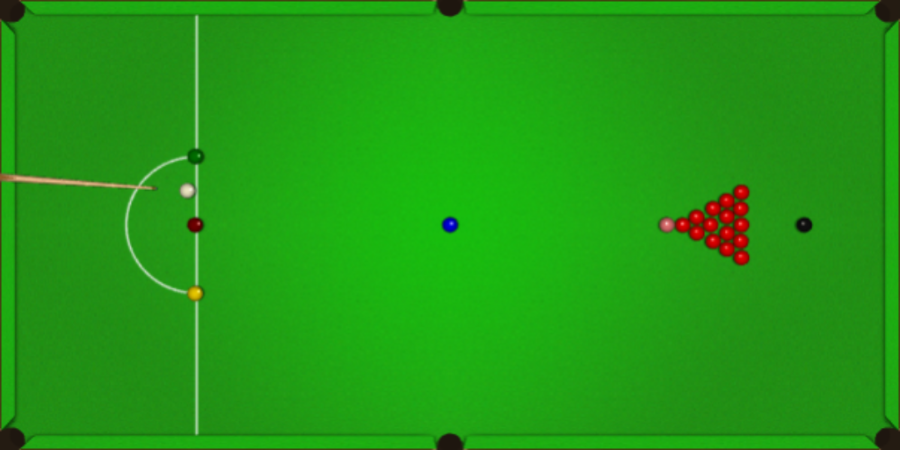
\includegraphics[width=100mm, keepaspectratio]{figures/starting_position.png}
    \caption{A golyók kezdeti pozíciója.}
    \label{fig:kezdeti_pozicio}
\end{figure}

\subsection{Pontszerzés}
A játékosok a pontjaikat a golyók bizonyos sorrendben való zsebbe helyezésével szerzik. Az egymás után hiba nélkül szerzett pontok összegét \textbf{törésnek} nevezzük. Egy játékos például szerzhet 9 pontos törést a következő golyók egymás utáni elhelyezésével \textit{piros -> zöld -> piros -> barna}.\cite{shamos2002new}
\par Egy játékos büntetőpontokat kap hibák elkövetése esetén. Hibát elkövetni lehet például a fehér golyó zsebbe helyezésével, nem megfelelő színű golyó elütésével. Az elkövetett hibáért minimum 4, maximum 7 pontlevonás jár, attól függően, hogy milyen színű golyók mozdulnak a hiba elkövetésekor (pl.: Ha a cél a piros golyó lelökése, de a lövő a feketét találja el, akkor 7 hibapont jár). A hibát elkövető játékos a törésének pontjait megkapja a hibát elkövetett lövés közben elhelyezett golyók pontjainak kivételével.\cite{snooker_rules}

\section{Az OpenCV képfeldolgozási könyvtár}
Az OpenCV egy főként \textbf{valós idejű képfeldolgozáshoz} használt programozási függvénykönyvtár. A könyvtár többféle programozási nyelvekhez készült implementációval létezik (pl.: C++, Python, Java stb.)\cite{opencv_2020}, ezek közül ebben a projektben Python programozási nyelven keresztül fogom használni.
\par A könyvtárból használt függvények segítségével kerülnek megnyitásra a képek, továbbá a képeken való műveletek (pl.: szürkeárnyalatolás, élkeresés) is a könyvtár segítségével lesznek végrehajtva. A későbbiekben lesz szó a könyvtárból használt függvényekről, azok működéséről nagyobb részletességben.

\section{Tensorflow a neurális hálózatokhoz}
A Tensorflow az OpenCV -hez hasonlóan egy függvénykönyvtár, azzal a különbséggel, hogy a könyvtár a \textbf{neurális hálózatok elkészítését és betanítását} teszi lehetővé.\cite{tensorflow} A neurális hálózatok közül itt főként neurális hálózatokat (Neural Network) fogok használni, amelyek a képfeldolgozás, kép osztályozás területén teljesítenek kiemelkedően. A könyvtár eszközeiről szintén részletesebben beszélek majd a későbbi fejezetekben.
\chapter{A golyók pozíciójának felismerése}
\section{A probléma ismertetése}
Ebben a fejezetben a címből is láthatóan az asztal és azon elhelyezkedő \textbf{golyók pozíciójának felismeréséről} lesz szó. A program ezen része bemenetként fog fogadni egy képet. Ez a kép származhat \textbf{videófelvételből} (videófelvétel egy képkockája), \textbf{valós idejű felvételből} (szintén egy képkocka), vagy szimplán egy \textbf{képfájlból}. A program készítése közben egy valósághű internetes snooker játékról\cite{flyordie} készített felvételeket fogok használni a felismeréshez. A videójátékból származó felvétel azonban bizonyos szempontokból eltér a valóságtól, ezekről később lesz szó, de lényegében jól használható a felismerés elkészítéséhez, továbbá megkönnyíti a tesztelést és a felvételek beszerzését. A bemenő adatot ezután képfelismerési folyamatok után a \ref{tab:felismert_koordinatak} táblázatban látható koordinátákra alakítjuk.

\begin{figure}[!ht]
    \centering
    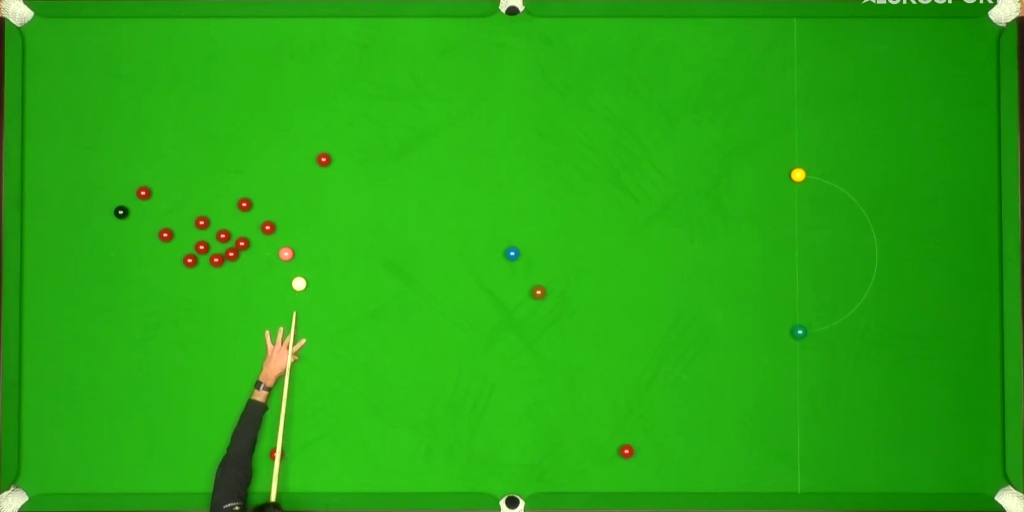
\includegraphics[width=100mm, keepaspectratio]{figures/input_table.png}
    \caption{Egy bemeneti kép az asztal felismerő lépés után.}
    \label{fig:bemeneti_asztal}
\end{figure}

\begin{table}[!ht]
    \caption{A golyó felismerés kimeneti adatai a \ref{fig:bemeneti_asztal} kép alapján.}
    \label{tab:felismert_koordinatak}
	\footnotesize
	\centering
	\begin{tabular}{ l l l }
		\toprule
		golyó színe & x pozíció (0 - 1024) & y pozíció (0 - 512) \\
		\midrule
		yellow & 156 & 176\\
        brown  & 224 & 254\\
        green  & 226 & 178\\
        red    & 460 & 480\\
        pink   & 464 & 344\\
        blue   & 514 & 256\\
        white  & 622 & 472\\
        red    & 698 & 324\\
        red    & 724 & 394\\
        red    & 896 & 250\\
        black  & 918 & 256\\
		\bottomrule
	\end{tabular}
\end{table}

\par A \ref{fig:bemeneti_asztal} képen már az asztal felismerés után való képet mutatom, a láthatóság megkönnyítése érdekében. A fejezet következő részeiben a bemeneti nyers képről koordinátákra való átalakítás lehetséges módszereit ismertetem lépésekre bontva.

\section{Az asztal felismerése}
Ez a lépés kicsit elkülönül a többi lépéstől, hiszen a további lépések különféle módszerektől függetlenül, megegyezően ezen a lépésen alapszanak. Ahhoz hogy a további lépések pontosak legyenek és megfeleő teljesítménnyel működjenek, az asztalt mindig azonos méretben, elforgatásban és torzításban kell megkapniuk.
\par Ebben a módszerben az elforgatáson kívül a detektálás, átméretezés és a torzítás lesz középpontban. Az elforgatást nem veszem figyelembe, hiszen a bemenetről elvárt, hogy bizonyos orientációban kapjuk meg. Tehát amit valójában kapunk függetlenül a bemenet megszerzésének módszerétől, a \ref{fig:bemeneti_kep} képen látható.

\begin{figure}[!ht]
    \centering
    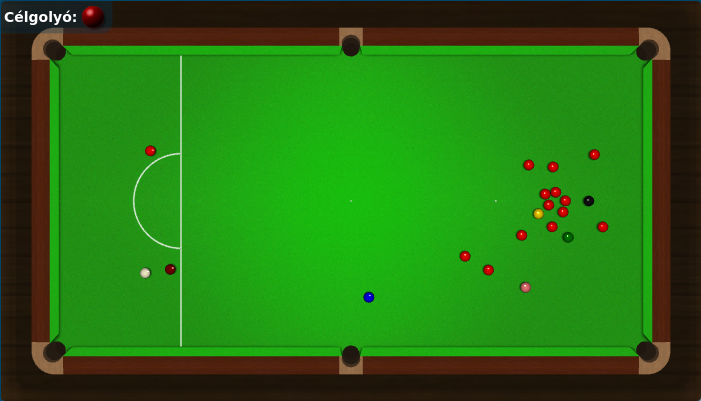
\includegraphics[width=150mm, keepaspectratio]{figures/input_screen.png}
    \caption{Egy nyers bemeneti kép a játék ablakáról.}
    \label{fig:bemeneti_kep}
\end{figure}

\par Ezen a képen kell megtalálnunk a játékterület zöld részét. Ezt megtehetjük, ha először is a képünket ún. HSV (Hue Saturation Value) formátumra alakítjuk. Ennek a konverziónak a kimenete a \ref{fig:bemeneti_kep_hsv} képen látható.

\begin{figure}[!ht]
    \centering
    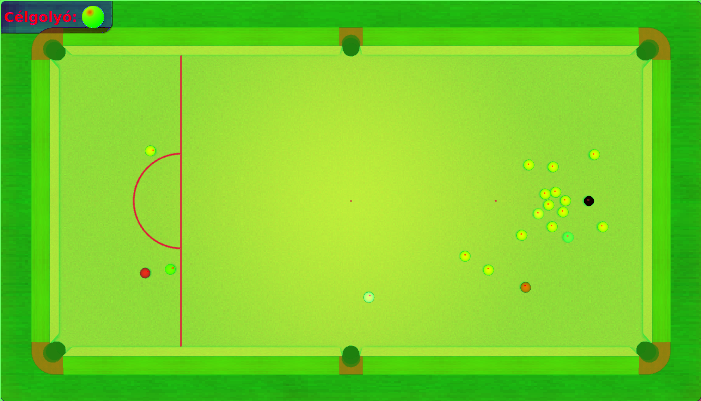
\includegraphics[width=150mm, keepaspectratio]{figures/input_screen_hsv.png}
    \caption{A \ref{fig:bemeneti_kep} kép HSV re alakított verziója RGB reprezentációban.}
    \label{fig:bemeneti_kep_hsv}
\end{figure}

\par Ez az átalakítás azért fontos, mert HSV formátumban könnyebben intervallumok közé lehet szorítani a játékterület zöld színét.
\newline Ezek az intervallumok:
\begin{itemize}
    \setlength\itemsep{-2pt}
    \item Árnyalat (Hue)
    \item Telítettség (Saturation)
    \item Érték (Value)
\end{itemize}
\par Az adott intervallum értékeken kívül helyezkedő értékeket maszkoljuk, és eredményül a kívánt zöld területeket kapjuk. Ezt a képet a maszkolás után visszaalakítjuk RGB formátumra. A folyamat után kapott kép a \ref{fig:bemeneti_kep_mask} képen látható.

\begin{figure}[!ht]
    \centering
    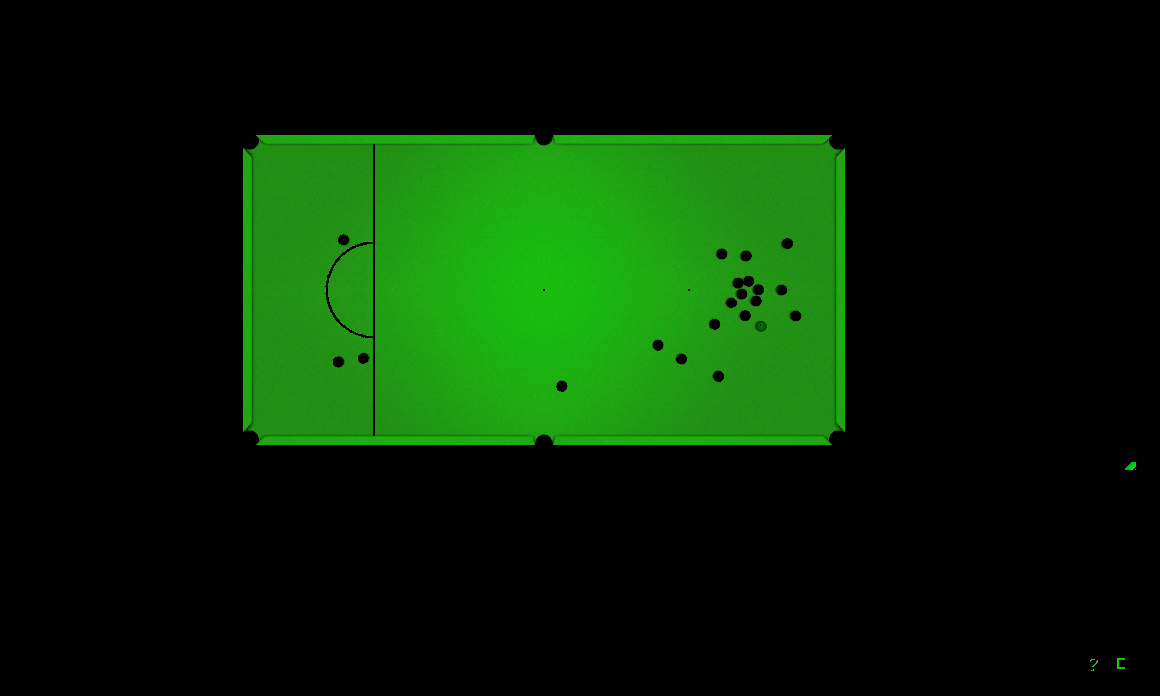
\includegraphics[width=150mm, keepaspectratio]{figures/input_screen_mask.png}
    \caption{A \ref{fig:bemeneti_kep} kép a maszkolás után.}
    \label{fig:bemeneti_kep_mask}
\end{figure}

\par Az előző folyamat után már jól látható a játékterület, azonban vannak apró foltok amik nem kerületk maszkolásra. Ezek a foltok hasonló HSV értékekkel rendelkeznek, mint a játékterület, kiszűrésük megoldható a kontúrok megkeresésével, majd feltételezve, hogy a legnagyobb folt a maszkolt képen a játékterület, annak kiválasztásával. Ezzel az eljárással már megadható a játékterület kontúrja. Feltételezve, hogy ez a négy sarokpontból áll, és egy téglalap pontosan határolja, a játékterület képe \ref{fig:bemeneti_asztal2} megkapható a kontúr eredeti képből való kivágásával és átméretezésével.

\begin{figure}[!ht]
    \centering
    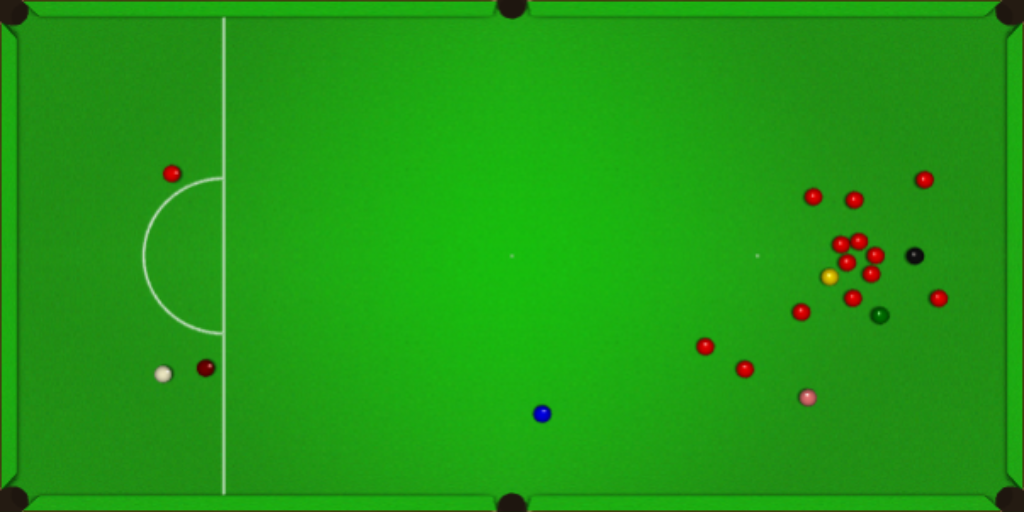
\includegraphics[width=100mm, keepaspectratio]{figures/input_table2.png}
    \caption{Az eredeti képből kinyert játékterület.}
    \label{fig:bemeneti_asztal2}
\end{figure}

\par Fent említettem, hogy feltételezhetjük, hogy a játékterület kontúrja a kontúrkeresés után téglalap alakú, és a kontúrt alkotó pontok száma 4. Viszont valóságban ez nehezen fordul elő, ezért szükséges a pontok számának leszűkítése és a négy pontot határoló alakzatban lévő kép torzítása 2:1 oldalarányú téglalapra. Az oldalarány a szabvány snookerasztal 12 x 6 láb (365,8 cm x 182,9 cm)\cite{snooker_rules} méretéből következik. A pontok szűkítéséről és a torzításról a megvalósítás fejezetben lesz részletesetbben szó.

\section{A golyók azonosítása}
A golyók azonosítását különféle mószerekkel végezhetjük el, ezek eltérnek sebességben és pontosságban. A folyamatok bemenete az előzőekben megismert asztal felismerés kimenete lesz, kimenetük pedig a \ref{tab:felismert_koordinatak} táblázatban látható x és y pozíciók, adott golyók színe szerint. A folyamat belső működése módszerenként eltér egymástól, ezeket a módszereket az implementáció egyes iterációjának részeként használtam, majd változtattam meg az elért teljesítmény növeléséhez.

\subsection{Azonosítás mintaillesztéssel}
Ennek a módszernek az alapja tisztán mintaillesztéssel működik. A mintaillesztés egy arányos méretű képet illeszt rá a játékterület képére, majd amennyiben az illeszkedés mértéke meghalad egy bizonyos küszöbértéket, a mintaillesztés iterációjának a pozíciója mentésre kerül. Ebből a pozícióból meghatározható a golyó helyzete. A mintaillesztéshez használt minta a \ref{fig:minta_kep} ábrán látható.

\begin{figure}[!ht]
    \centering
    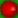
\includegraphics[width=30mm, keepaspectratio]{figures/template_red.png}
    \caption{A mintaillesztéshez használt minta.}
    \label{fig:minta_kep}
\end{figure}

\par A \ref{fig:minta_kep} minta felbontása láthatóan alacsony, azonban túl nagy felbontás esetén a folyamat meglehetősen lassabban megy végbe, továbbá a minta méretét még a felismert játékterület mérete is meghatározza.
\par A mintaillesztés ún. Kereszt Korrelációval (Normed Cross Correlation) megy végbe, ezt a \ref{for:cross_correlation} képletben láthatjuk\cite{kaehler2016learning, opencv_docs}.

\begin{equation}
    R(x, y) = \frac{\sum_{x',y'}(T(x',y') \cdot I(x + x', y + y'))}{\sqrt{\sum_{x',y'}T(x',y')^2 \cdot \sum_{x',y'}I(x + x',y + y')^2}}
    \label{for:cross_correlation}
\end{equation}

\par A képletben az $x$ és $y$ az eredeti képen vizsgált terület bal felső sarkát, $x'$ és $y'$ a minta képnek az adott képpontját, $T$ a minta képet és $I$ az eredeti képet jelöli.
\par A mintaillesztés problémái közé tartozik, hogy a zöld golyó mintaillesztésénél a küszöbérték et beállítani nehéz, és az eredmény pontatlan, lásd \ref{fig:rossz_zold}.

\begin{figure}[!ht]
    \centering
    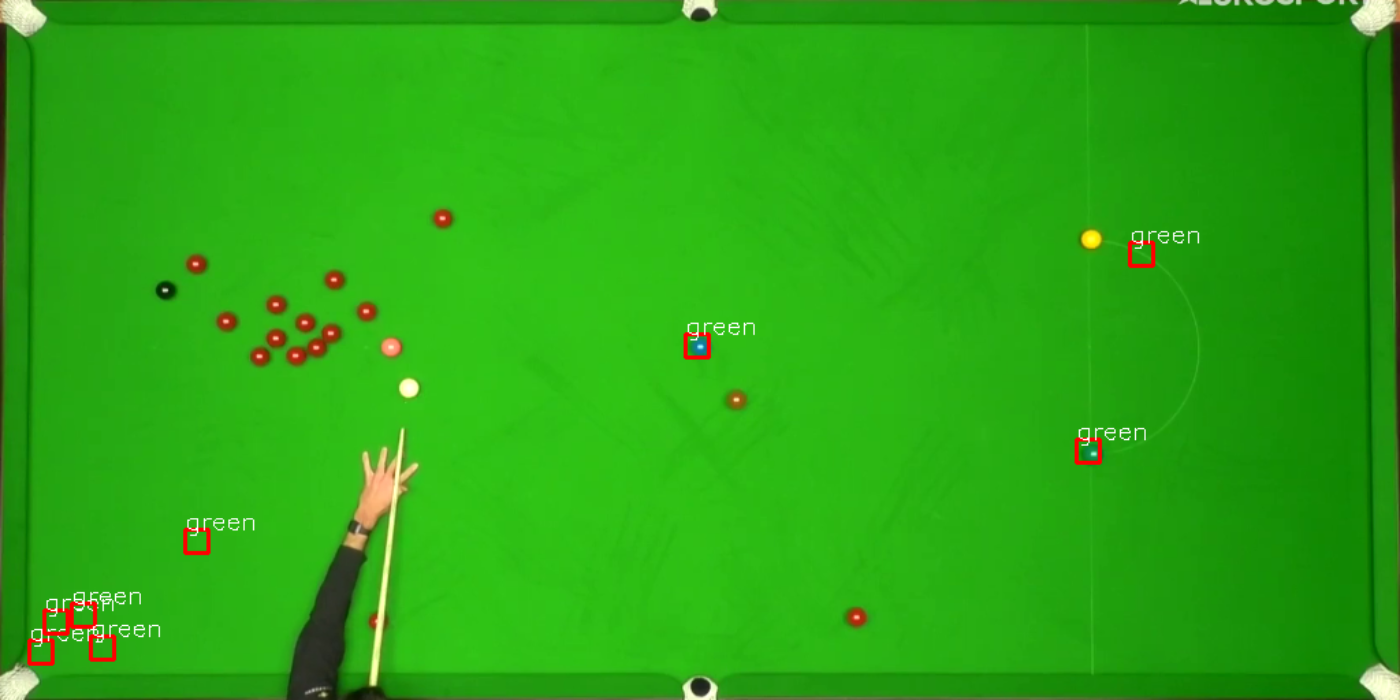
\includegraphics[width=73mm, keepaspectratio]{figures/wrong_green.png}\hspace{2mm}
	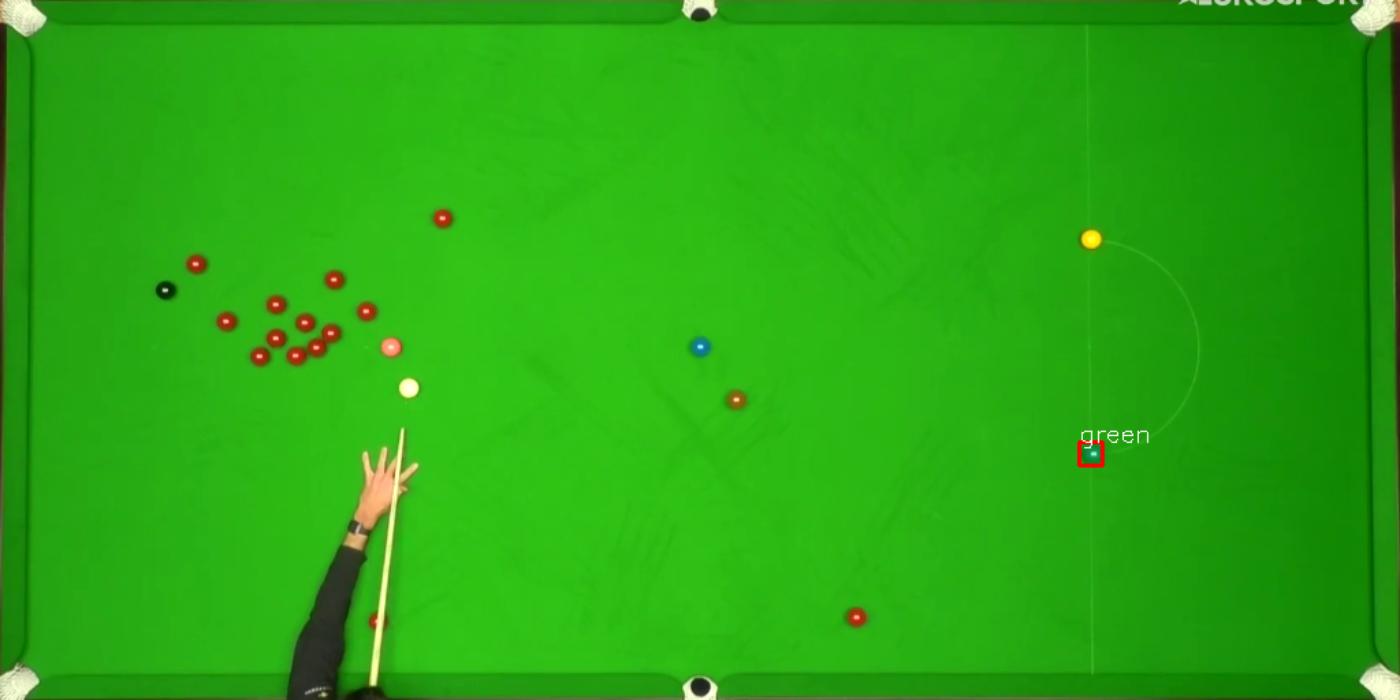
\includegraphics[width=73mm, keepaspectratio]{figures/green_ok.png}\\\vspace{5mm}
    \caption{A zöld golyó mintaillesztésének hibája (bal) és annak orvoslása HSV konverzióval (jobb).}
    \label{fig:rossz_zold}
\end{figure}

\par A \ref{fig:rossz_zold} ábrán látható hiba valamelyes orvosolható a kép és minta HSV -re való konvertálásával. Ez a konverzió jó eredményeket ad, azonban nagyon minimálisan csökkenti a teljesítményt. A mintaillesztés sajnos prolémákba ütközik a piros és barna golyók megkülönböztetésekor is. Ez a \ref{fig:rossz_barna} képen látható.

\begin{figure}[!ht]
    \centering
    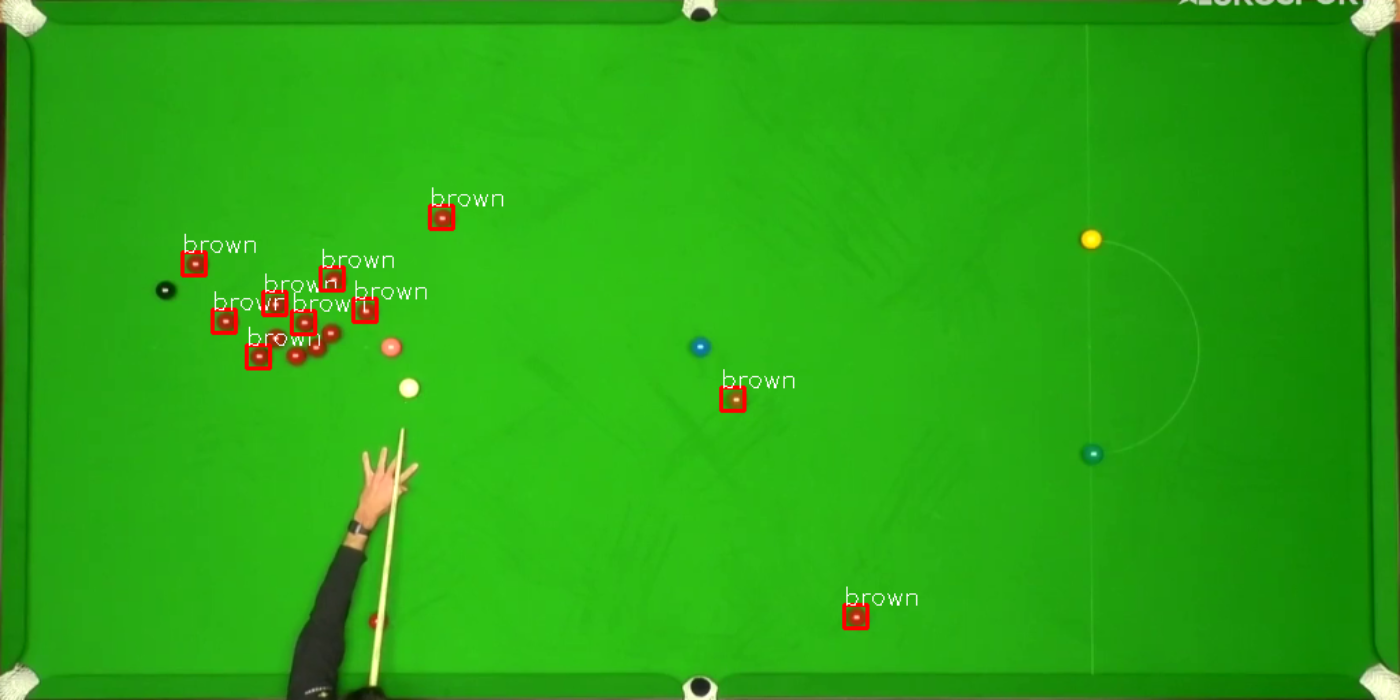
\includegraphics[width=73mm, keepaspectratio]{figures/wrong_brown.png}\hspace{2mm}
	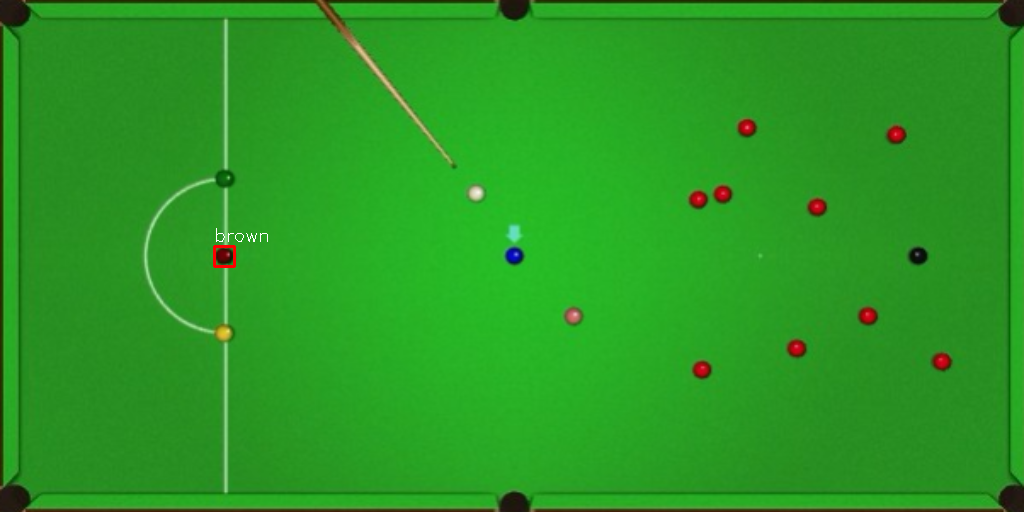
\includegraphics[width=73mm, keepaspectratio]{figures/brown_ok.png}\\\vspace{5mm}
    \caption{A barna golyó mintaillesztésének hibája (bal) és annak orvoslása a piros golyók levonásával (jobb).}
    \label{fig:rossz_barna}
\end{figure}

\par Itt a színek közelsége miatt nehéz megkülönböztetni a golyókat, ezért a piros és barna golyók nagyon minimálisan térnek el a \ref{for:cross_correlation} függvény miatt. Ez a probléma HSV konvertálás után is fennáll. Erre a megoldás, hogy az érzékelt piros golyók kivonásra kerülnek a barna golyók listájából. Ahhoz, hogy pontos legyen az eredmény, viszont szükséges, hogy a piros golyók megfelelően legyenek érzékelve, amely nem minden esetben biztosítható, ezért ez a módszer nem túl pontos bizonyos bemenetekre. Hasonló problémák merülhetnek fel a piros és rózsaszín, továbbá a fehér és rózsaszín golyók felismerésekor is.
\par Annak ellenére, hogy a módszer nem túl optimális, jól használható adatkészeletek készítésére, hiszen a felsmerést nagyrészt helyesen megoldja és a problémák ismeretében a kézzel válogatást nagymértékben megkönnyíti.

\subsection{Azonosítás körkeresés és mintaillesztéssel}
Az előző módszerhez hasonlóan a golyó színek szerinti osztályozása itt is mintaillesztéssel történik, azonban a sebesség növelése érdekében itt először a golyókat kördetektálással azonosítjuk, majd ennek eredményét adjuk át a mintaillesztő algoritmusnak. Ez az egész képen való pásztázás és mintaillesztéshez képest a teljesítményt a minták leszűkített mennyiségével nagymértékben növeli.

\par A körök detektálásához az ún. Hough transzformációt (Hough Transformation) fogom használni, ez a H.K. Yuen, J. Princen, J. Illingworth és J. Kittler et. al. 1990 \cite{YUEN199071} szerint abban az esetben, ha egy kör a kövekező \ref{for:hough_transform} függvénnyel írható le,

\begin{equation}
    (x - a)^2 + (y - b)^2 = r^2
    \label{for:hough_transform}
\end{equation}

\par ahol $a$ és $b$ a kör középpontjának koordinátái és $r$ a sugár, akkor a körvonal élének egy tetszőleges $x_i$, $y_i$ pontja átalakításra kerül egy $a$, $b$, $r$ paraméterek által meghatározott térben elhelyezkedő egyenes kör alapú kúppá.\cite{hough_transform,YUEN199071} Amennyiben az adott pontok egy körvonalon helyezkednek el, a kúpok metszeni fogják egymást a kör $a$, $b$, $r$ pontjainak megfelelően.\cite{YUEN199071}
\par A körök megtalálásához az algoritmusnak meg kell adni néhány paramétert, ezek közé tartozhat:
\begin{itemize}
    \setlength\itemsep{-2pt}
    \item A keresett körök minimális és maximális sugara
    \item A keresett körök közti minimális távolság, duplikációk szűréséhez
    \item Az ellenőrzött alakzatok körrel való hasonlóságának küszöbértéke
\end{itemize}
\par Az algoritmus lefutása után megkapjuk a bemeneti játékterületen talált kör alakú kontúrokat. Ezt a \ref{fig:talalt_korok} ábra szemlélteti.

\begin{figure}[!ht]
    \centering
    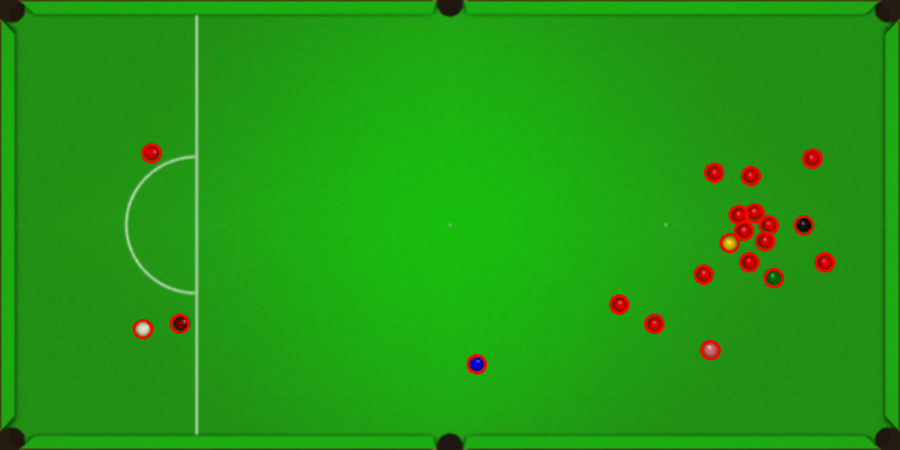
\includegraphics[width=100mm, keepaspectratio]{figures/detected_circles.png}
    \caption{A Hough transzformáció lefutása után kapott körök.}
    \label{fig:talalt_korok}
\end{figure}

\par Ez a módszer körök megtalálására jól használható, a mintaillesztéshez szükséges képek könnyedén kivághatók az eredeti képből a körök paraméterei alapján. A probléma szintén a mintaillesztéssel van, hiszen a kivágott körök az előzőleg megismert mintaillesztéssel kerülnek beazonosításra. Ez sajnos az eddig megismert hibákat vonja maga után, annak ellenére, hogy a sebesség javul. Viszont akárcsak a szimpla mintaillesztéses módszer ez a módszer is alkalmas adatkészletek elkészítésére, és a kapott adatok kézzel ellenőrzését nagymértékben megkönnyíti.

\subsection{Azonosítás körkeresés és gépi tanulás segítségével}
Ahhoz, hogy kiküszöböljük a mintaillesztés hibáit, az osztályozást elvégezhetjük neurális hálózat segítségével. Ezt megtehetjük ugyancsak, ha egy kerettel végigpásztázunk a játékterület képén, de a körkereséses módszernél megismert Hough transzformációval jobb eredményt is elérhetünk. A következőkben a körkeresés eredményeképp kapott, a bemeneti játékterület képéből kivágott golyók osztályozásáról lesz szó neurális hálózat segítségével. A kivágott képek fogják a bemenetet képezni, majd a neurális hálózat azt osztályozza egy 0 tól 7 ig terjedő egész számként. Ezek a számok a golyók színeit reprezentálják, lásd \ref{tab:golyo_azonositok} táblázat.

\begin{table}[!ht]
    \caption{A golyók szín szerint, és azok azonosítói.}
    \label{tab:golyo_azonositok}
	\footnotesize
	\centering
	\begin{tabular}{ l c }
		\toprule
		Golyó színe & Azonosító \\
		\midrule
		fekete      & 0\\
        kék         & 1\\
        barna       & 2\\
        zöld        & 3\\
        rózsaszín   & 4\\
        piros       & 5\\
        fehér       & 6\\
        sárga       & 7\\
		\bottomrule
	\end{tabular}
\end{table}

\par A neurális hálózat betanításához szükség van betanítási adatkészletre, viszont az előzőekben megsimert módszereknél szóba került, hogy viszonylag kevés kézi szortírozással könnyedén lehet velül előállítani adatkészletet, amely tökéletes a neurális hálózat betanításához és teszteléséhez. Az adatkészlet néhány eleme látható a \ref{fig:adatkeszlet} ábrán.

\begin{figure}[!ht]
    \centering
    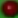
\includegraphics[width=30mm, keepaspectratio]{figures/dataset_1.png}\hspace{5mm}
    
\includegraphics[width=30mm, keepaspectratio]{figures/dataset_2.png}\hspace{5mm}
	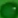
\includegraphics[width=30mm, keepaspectratio]{figures/dataset_3.png}\\\vspace{5mm}
    
\includegraphics[width=30mm, keepaspectratio]{figures/dataset_4.png}\hspace{5mm}
    
\includegraphics[width=30mm, keepaspectratio]{figures/dataset_5.png}\hspace{5mm}
	
\includegraphics[width=30mm, keepaspectratio]{figures/dataset_6.png}\\\vspace{5mm}
    \caption{Az adatkészlet elemei.}
    \label{fig:adatkeszlet}
\end{figure}

\par A betöltött adatokat megfelelően azonosítva címkéjük szerint, átadjuk a neurális hálózatnak. Ahhoz, hogy a tanítás jó eredményeket hozzon, gondoskodni kell arról, hogy a betanítási adatok közt egyenlő arányban szerepelnek az egyes golyók színek szerint, továbbá, hogy az adatkészlet elemei megfelelően össze vannak keverve. Az előkészített adatkészlet egy kis részét (10\% - 30\%) elkülönítjük, majd ezt használjuk a neurális hálózat pontosságának tesztelésére.
\par A betanítási folyamatok után elmentjük a neurális hálózatot, majd amikor használni szeretnénk, csak be kell tölteni. A tanítás és felhasználás külön programfájlokban könnyedén elvégezhető.
\par A körfelismerés módszerrel ötvözve, a neurális hálózattal való osztályozás gyors és pontos eredményeket biztosít. A felismerés egy kimenetele a \ref{fig:felismert_asztal} képen látható.

\begin{figure}[!ht]
    \centering
    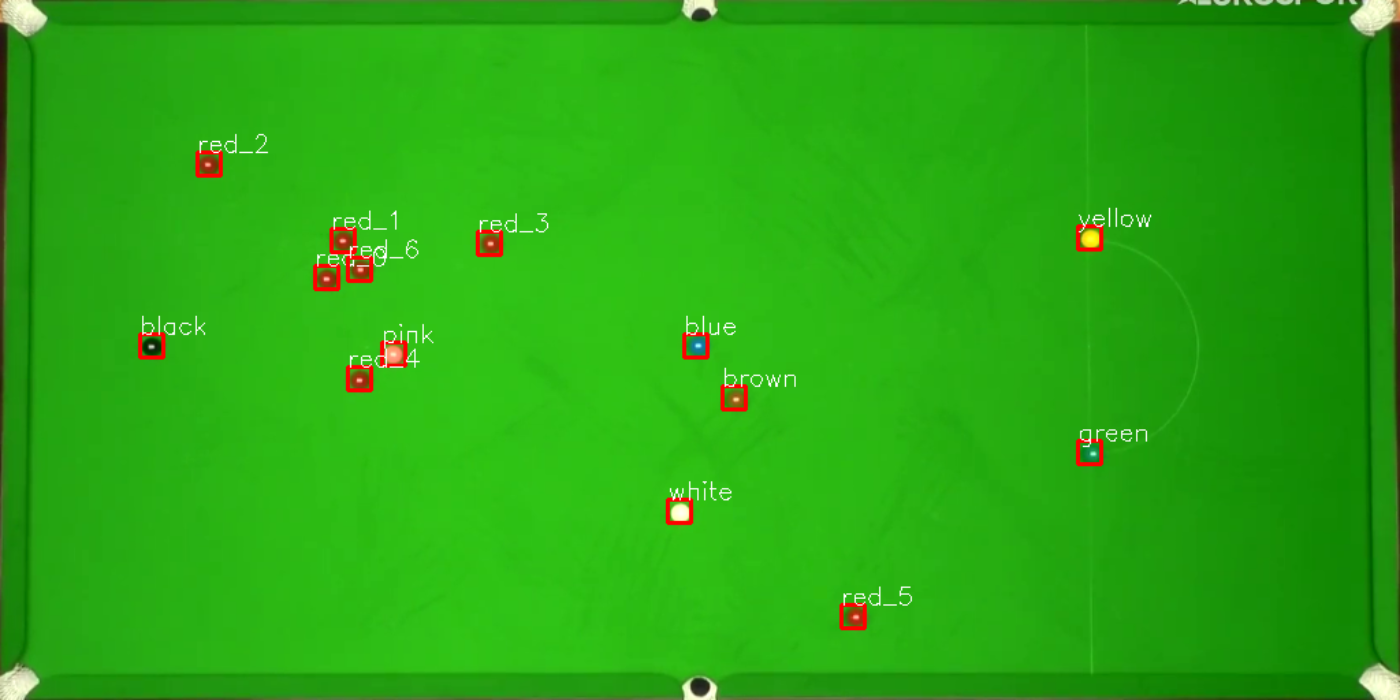
\includegraphics[width=100mm, keepaspectratio]{figures/recognised_table.png}
    \caption{A neurális hálózattal való golyófelismerés kimenete.}
    \label{fig:felismert_asztal}
\end{figure}

\par A módszer eredményességének köszönhetően későbbiekben részletesebben ismertetem a megvalósítás fejezetben.
\chapter{Analizálás}
\chapter{Megvalósítás}
\section{Alkalmazott módszerek}
A megvalósítás során az eddig megismert módszereket fogom felhasználni, azokat Python programozási nyelven fogom elkészíteni és ismertetni. Az egyes algoritmusokat függvények formájában készítem el, ezeket a függvényeket pedig több Python szkriptben is felhasználom.
\par Az eddig megismert módszerek közül elsősorban a nyers bemenetből emelem ki a játékterületet, ezt követően a golyók pozíciójának felismeréséhez kör detektálást és egy neurális hálózatot fogok használni. A neurális hálózat betanításához az adatkészletet kör detektálással, mintaillesztéssel és kézi válogatással fogom elkészíteni. A következőkben az egyes függvények működését, azokban felhasznált külső könyvtárak eszközeit ismertetem részleteiben.
\par A fejezetek felosztása az eddig megismert lépések szerint kerül rendezésre.

\section{A golyók pozíciója}

\subsection{A szükséges könyvtárak importálása}
Ahhoz hogy a függvények megfeleően működjenek, meg kell mondanunk a programnak, hogy használja a külső könyvtárakat.
\newline Ezt a következőképp tehetjük meg.

\vspace{2mm}\begin{lstlisting}[language=Python, numbers=left]
import math
import numpy as np
import cv2
\end{lstlisting}

\par A \lstinline{math} könyvtár segítségével matematikai műveleteket (gyökvonás, szinusz, koszinusz) tudunk végezni, a \lstinline{numpy} könyvtár a tömbök, mátrixok kezelését, azokkal való műveleteket segíti és gyorsítja, a \lstinline{cv2} pedig az OpenCV eszközeit teszi elérhetővé.

\subsection{Az asztal kivágása}
Annak érdekében, hogy a nyers képből kinyerjük a játékterületet, azt először be kell tölteni egy többdimenziós tömbbe. A kép betöltése többféleképp végbemehet, ezért ezt konkrétan nem részletezem.
\par A betöltött kép tömbjének alakja megegyezik a kép szélességével és magasságával, továbbá az intenzitási értékekkel, tehát ha betöltünk egy 1024 x 512 méretű RGB képet, annak tömbjének az első és második dimenziója 1024 és 512, a harmadik pedig az RGB (Piros, Zöld, Kék) intenzitásoknak megfelelően 3 méretű.
\par Fontos megjegyezni, hogy az OpenCV a képeket betöltéskor BGR formátumban tölti be, ez az elnevezésből adódóan annyiban tér el az RGB formátumtól, hogy a piros (R) és kék (B) színcsatornák fel vannak cserélve.
\par A nyers bemeneti kép megszerzése után készen állunk az asztal megkeresésére és kivágására. Első lépésként a képet átalakítjuk HSV formátumra, majd megadjuk az alsó és felső intenzitási értékhatárokat, amelyből elkészítjük a maszkot. Ezután maszkoljuk az eredeti képet a maszk segítségével.
\newline Ezt a következő kódsorokkal végezhetjük el.


\vspace{2mm}\begin{lstlisting}[language=Python, numbers=left]
hsv = cv2.cvtColor(image, cv2.COLOR_BGR2HSV)

lower_green = np.array([40, 190, 50])
upper_green = np.array([65, 255, 225])

mask = cv2.inRange(hsv, lower_green, upper_green)

result = cv2.bitwise_and(image, image, mask = mask)
\end{lstlisting}

\par A kódban az \lstinline{image} a bemeneti képünk, amelyet a \lstinline{cv2.cvtColor} függvénnyel \cite{cv2_cvt_color} konvertálunk át HSV formátumra. Ennek a függvénynek az első paramétere a bemeneti képünk, a második pedig a konverzió típusa, amely ebben az esetben BGR $\rightarrow$ HSV. A \lstinline{lower_green} és \lstinline{upper_green} változók az alsó és felső intenzitási határokat jelölik sorrendnek megfelelően. A maszk elkészítését a \lstinline{cv2.inRange} függvénnyel \cite{cv2_in_range} végezhetjük el itt a paraméterek sorban a HSV re konvertált képünk, valamint az alsó és felső intenzitás értékek.
\newline A függvény a következők alapján dönti el, a maszk intenzitását,

\begin{equation}
    M(I) = L(I) \le S(I) \le U(I)
    \label{for:maszkolas}
\end{equation}

\par ahol $M$ a maszk, $L$ az alsó, $U$ a felső és $S$ a bemeneti HSV képet jelöli. A \ref{for:maszkolas} függvény mindhárom intenzitásra alkalmazásra kerül, a maszkban az intervallumon belüli intenzitások 255, a kívüliek pedig 0 értéket kapnak. A maszk elkészítése után azt alkalmazzuk az eredeti bemenő képre a \lstinline{cv2.bitwise_and} függvény \cite{cv2_bitwise_and} segítségével. Itt a paraméterek a bejövő eredeti kép \lstinline{image} kétszer és a maszk \lstinline{mask}.
\newline A folyamat során a metódus a következőképp jár el,

\begin{equation}
    R(I) = S_1(I)\quad \land\quad S_2(I)\qquad ,ha\quad M(I) \ne 0
    \label{for:maszk_alkalmazas}
\end{equation}

\par ahol $R$ a kimenő maszkolt kép (\lstinline{result}) $S_1$ és $S_2$ a két bemeneti kép paraméter, és $M$ a maszk. A bemenetben a kép azért szerepel kétszer egymás után, mert a \ref{for:maszk_alkalmazas} függvényben láthatóan a két bemenő paraméter közt egy bit szintű 'és' művelet történik, amennyiben a maszk nem nulla. Ez azt teszi lehetővé, hogy az eredeti képet kapjuk a maszkolt elemek kivételével, ami azért történik, mert bit szinten ha két megegyező elem közt történik 'és' művelet, akkor az eredmény szintén megegyezik a két elemmel. Ennek a folyamatnak a kimenetele látható a már előzőleg tárgyalt \ref{fig:bemeneti_kep_mask} ábrán.
\par A maszkolt kép megszerzése után elvégezhetjük az éldetektálást, amelyet megelőz egy szürkeárnyalatolás.
\newline Ezeket a műveleteket a következő programsorokkal végezhetjük.

\vspace{2mm}\begin{lstlisting}[language=Python, numbers=left]
image_gray = cv2.cvtColor(result, cv2.COLOR_BGR2GRAY)

result = cv2.Canny(image_gray, 100, 200)
\end{lstlisting}

\par A szürkeárnyalati konverziót a már megismert \lstinline{cv2.cvtColor} függvénnyel \cite{cv2_cvt_color} végezzük el, majd ezután megkeressük az éleket a képen Canny éldetektálás \cite{cv2_canny,canny_edge_detection} (\lstinline{cv2.Canny}) segítségével.
\newline A Canny éldetektálás általában több lépésre bontható szét, ezek lehetnek:

\begin{itemize}
    \setlength\itemsep{-2pt}
    \item Homályosítás Gauss szűrővel \cite{shapiro2001} a zajcsökkentés érdekében
    \item Élek helyének és irányának megállapítása intenzitás-gradiensből
    \item Nem-Maximum vágás merőleges élek szűréshéhez
    \item Kettős küszöbölés élek szűréséhez
\end{itemize}

\par Az éldetektálásnál meg kell adnunk a függvénynek a szürkeárnyalatos képünket, továbbá két küszöbértéket, amelyet a Canny detektálás a kettős küszöbölés folyamat során fog felhasználni. Itt, ha a felső küszöb felett van egy potenciális él, azt felvesszük az élek közé, ha az alsó küszöb alatt van eldobjuk és ha a felső és alsó küszöbök közt helyezkedik el, akkor a szomszédos pixelek alapján vesszük fel élnek. Az éldetektálással kapott kép a \ref{fig:bemeneti_kep_edge} ábrán látható.

\begin{figure}[!ht]
    \centering
    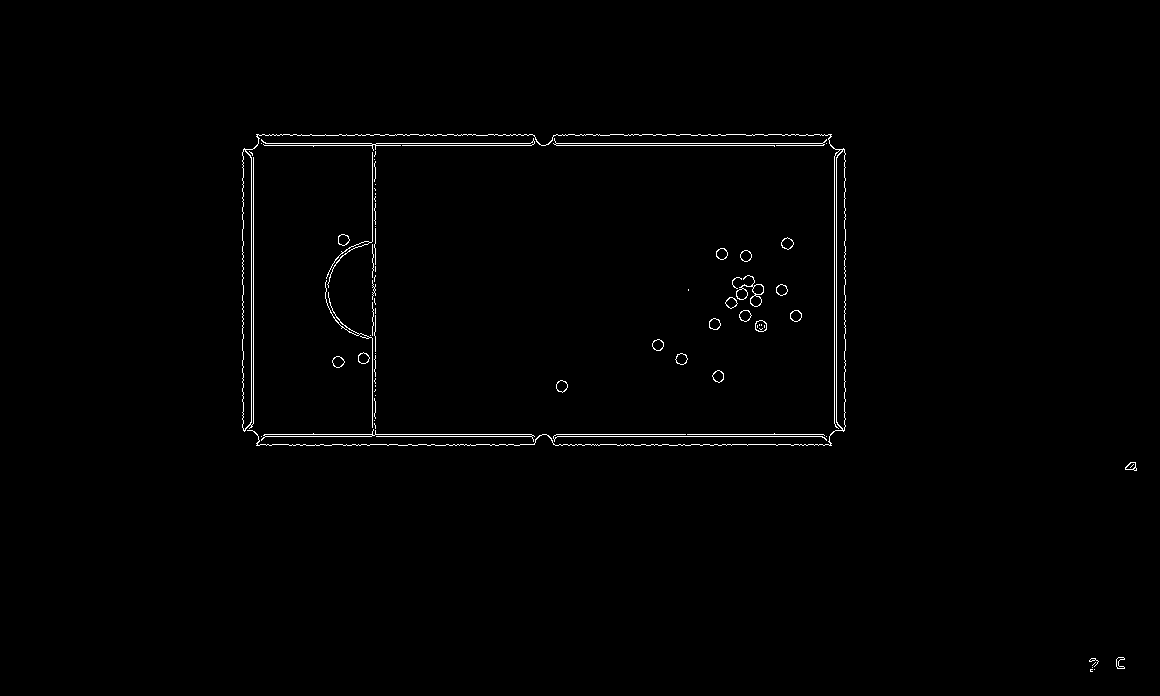
\includegraphics[width=150mm, keepaspectratio]{figures/input_screen_edge.png}
    \caption{A Canny éldetektálás után kapott kép.}
    \label{fig:bemeneti_kep_edge}
\end{figure}
%\include{content/introduction}
%\include{content/thesis-format}
%\include{content/latex-tools}
%\include{content/template-usage}


% Köszönetnyilvánítás - opcionális
%~~~~~~~~~~~~~~~~~~~~~~~~~~~~~~~~~~~~~~~~~~~~~~~~~~~~~~~~~~~~~~~~~~~~~~~~~~~~~~~~~~~~~~
%%----------------------------------------------------------------------------
\chapter*{\koszonetnyilvanitas}\addcontentsline{toc}{chapter}{\koszonetnyilvanitas}
%----------------------------------------------------------------------------

Ez nem kötelező, akár törölhető is. Ha a szerző szükségét érzi, itt lehet köszönetet nyilvánítani azoknak, akik hozzájárultak munkájukkal ahhoz, hogy a hallgató a szakdolgozatban vagy diplomamunkában leírt feladatokat sikeresen elvégezze. A konzulensnek való köszönetnyilvánítás sem kötelező, a konzulensnek hivatalosan is dolga, hogy a hallgatót konzultálja.


% Ábrák listája - a word-ös sablon szerint szükséges
%~~~~~~~~~~~~~~~~~~~~~~~~~~~~~~~~~~~~~~~~~~~~~~~~~~~~~~~~~~~~~~~~~~~~~~~~~~~~~~~~~~~~~~
\clearpage\phantomsection
\listoffigures
\addcontentsline{toc}{chapter}{\listfigurename}


% Táblázatok listája - opcionális
%~~~~~~~~~~~~~~~~~~~~~~~~~~~~~~~~~~~~~~~~~~~~~~~~~~~~~~~~~~~~~~~~~~~~~~~~~~~~~~~~~~~~~~
%\clearpage\phantomsection
%\listoftables
%\addcontentsline{toc}{chapter}{\listtablename}


% Irodalomjegyzék
%~~~~~~~~~~~~~~~~~~~~~~~~~~~~~~~~~~~~~~~~~~~~~~~~~~~~~~~~~~~~~~~~~~~~~~~~~~~~~~~~~~~~~~
\clearpage\phantomsection
\bibliography{bib/mybib}
\addcontentsline{toc}{chapter}{\bibname}


% Függelékek
%~~~~~~~~~~~~~~~~~~~~~~~~~~~~~~~~~~~~~~~~~~~~~~~~~~~~~~~~~~~~~~~~~~~~~~~~~~~~~~~~~~~~~~
%%----------------------------------------------------------------------------
\appendix
%----------------------------------------------------------------------------
\chapter*{\fuggelek}\addcontentsline{toc}{chapter}{\fuggelek}
\setcounter{chapter}{\appendixnumber}
%\setcounter{equation}{0} % a fofejezet-szamlalo az angol ABC 6. betuje (F) lesz
\numberwithin{equation}{section}
\numberwithin{figure}{section}
\numberwithin{lstlisting}{section}
%\numberwithin{tabular}{section}

\section{dataset5}
A betanításhoz használt adatkészlet, színenként külön mappákba helyezve, összesen nagyjából 12000 képfájlt tartalmaz.

\section{train2.py}
A neurális hálózat betanításához használt Python szkript.

\section{Cut.hpp}
A kivágott képek kezeléséhez létrehozott osztályt tartalmazó fájl.

\section{Section.hpp}
A szakaszok kezeléséhez létrehozott osztályt tartalmazó fájl.

\section{BallLabel.hpp}
A golyók színének enum értékeit tartalmazó fájl.

\section{Template.hpp}
A mintaillesztés során használt mintákhoz létrehozott osztály fájlja.

\section{Ball.hpp és Ball.cpp}
A golyókat és azok függvényeit tartalmazó osztály header fájlja és implementációja.

\section{Recognition.hpp és Recognition.cpp}
A felismerési folyamatok függvényeit tartalmazó forrásfájl header deklaráció és implementáció.

\section{TrackbarWindow.hpp}
A finomhangolási paraméterek megjelenítéséhez használt segédosztály fájlja.

\section{main.cpp}
A felismerő fő folyamatait egybefoglaló központi forráskód. A felismerés folyamatához használt többi programrész ebből a fájlból kerül meghívásra.

%\label{page:last}
\end{document}
